\section{Introduction}
In this chapter we expose the motivations that lead us to conduct this work, in particular, we analyze the current problems in the NoSQL service implementation of the CPIM library and propose a solution to address them and, at the same time, increasing the number of NoSQL database supported by the library.
\noindent Furthermore, we will discuss why we decided to include the possibility for the CPIM library users to be able to migrate and synchronize data, across databases, by means of a migration system called \textit{Hegira}.

\section{CPIM library extension}
The CPIM library achieve the objective of making a developer able to interact with many different services in the cloud. Due to modern application requirements in handling large volumes of data, CPIM should be extended, primarily in order to let it support more NoSQL technologies; indeed, the great diversity of the various NoSQL solutions makes curtains solutions more suitable than others in handling certain types of data. Hence, the possibility of choosing among many different NoSQL solution and, at the same time, be able to interact with them through a common interface, is an important feature to be added in CPIM. 

\subsection{CPIM NoSQL service}
The CPIM library uses various implementation of the JPA interface to ease the communication with different NoSQL databases:
\begin{itemize}
\item Google Datastore is supported by means of the Google JPA implementation around Datastore API;
\item Azure Tables is supported through \textit{jpa4azure} a third party implementation of the JPA interface for Tables;
\item Amazon Simple DB is supported through \textit{simpleJPA} a third party implementation of the JPA interface for Simple DB.
\end{itemize}
\noindent By choosing the cloud provider inside the \textit{configuration.xml}, the library knows, at run-time, which interface should be used for the service and this holds also for the NoSQL service. Hence to use Google Datastore as NoSQL database, Google must be selected as cloud provider.

\newparagraph The aim of CPIM is to offer to the user a way of writing cloud application in a provider-independent fashion, to be able to migrate the application from a provider to another without the necessity of re-engineer the application. For the NoSQL service this is achieved by meas of the JPA interface that, beside the fact that is is not a standard for accessing NoSQLs, many projects came into play trying to bring the benefit of the JPA interface also in the NoSQL world. 

\noindent However the current implementation have significant problems:
\begin{enumerate}
\item[\textbf{P.1}] the application code written to interact with the NoSQL service is not interoperable and thus, the user is required to modify the application code in order to be able to move the application to a different cloud provider.  
\end{enumerate}
\noindent Moreover the NoSQL service suffer of some limitations too:
\begin{enumerate}
\item[\textbf{L.1}] the choice of the NoSQL database is strictly bind to the selected cloud provider; 
\item[\textbf{L.2}] even if the selection of the NoSQL database would be possible, the number of supported NoSQL database is very limited.
\end{enumerate}

\noindent For \textbf{P.1}, the problem reside in the fact that for each of the currently supported database, has been found and integrated into CPIM, a specific implementation of the JPA interface. Even through JPA is a well defined standard, not every JPA provider follows strictly the specification and thus, different provider can behave differently while persisting the same entities, since they interpret differently the semantic of some JPA annotation.

\noindent An example of this problem is how Collection fields are currently handled in CPIM. In the Google JPA implementation for Datastore and in the JPA implementation for Amazon SimpleDB, Collection fields are handled correctly, with respect to the JPA specification, thought the \texttt{@ElementCollection} annotation, while, in the JPA implementation for Azure Tables, Collection fields needs to be annotated with the \texttt{@Embedded} annotation. This require a modification of the code and thus eliminates the effort of CPIM in achieving code portability among PaaS.

\newparagraph As regards \textbf{L.1} and \textbf{L.2}, we would like to  give to the user the ability to persist data in the database that best fit his requirements. For example if the user application will generate data that should be processed with Hadoop, the best solution is to store those data in an HBase instance since its integrate easily in Hadoop. Therefore we want to make the user able to persist different entities in different datastore based on his needs and without the limitation of a specific NoSQL technology.

\subsection{Proposed solution}
The proposed solution is mainly about the integration of Kundera, a JPA compliant ORM for NoSQL databases, as unique persistence layer for the NoSQL service. 

\noindent There are many reasons why we choose to use Kundera among the other available solutions in the scenario of NoSQLs common language. The main reason is that Kundera, through the use of the JPA interface will permit to the user to handle the complexity of NoSQL databases with expertise he already uses for SQL systems. Furthermore Kundera is in the field from 2010 and thus have a big and active community, built in many years of activity, and has been used successfully in some production environment. Furthermore its implementation of \textit{polyglot persistency} permits the development of complex applications that can potentially use many different NoSQL technologies at once.

\noindent The only drawback of using Kundera is that it does not support any of the NoSQL datastore currently supported by CPIM. Fortunately Kundera have, as its primary goal, to make the library as much extensible as possible, to let developers build their own client around new NoSQL technologies. The solution will thus be to contribute to Kundera as an open source project by developing two new Kundera clients, one for support Google Datastore and the other to support Azure Tables.

\newparagraph This integration will be useful to solve the problems and mitigate the limitation outlined as follow:
\begin{itemize}
\item since Kundera will be the unique persistence provider for the library we will relay only on one implementation of the JPA interface overtaking in this way, the problem \textbf{P.1}, related to different interpretation of the JPA annotation, and thus achieving complete portability of the code of the application model since no code modifications are required to work with different NoSQL database through Kundera;
\item the integration of Kundera permits a redesign of the NoSQL service aimed to decouple the chosen PaaS provider and the NoSQL technology overcoming limitation \textbf{L.1}, by giving to the user the ability of deciding which technology is more suitable for his needs. Furthermore exploiting the polyglot-persistence provided by Kundera, the user will be able to persist entities within different NoSQL databases at the same time, simply by defining accordingly the persistence unit in the \textit{persistence.xml} file;
\item choosing Kundera as persistence layer we can actually take advantage of the already developed extension for many different NoSQL databases, adding as a result the support of those database to CPIM, and thus overcoming the limitation \textbf{L.2}.
\end{itemize}

\section{Data migration}
NoSQL technologies do not offer a common querying language to interact with them, as SQL does for RDBMS. Furthermore, NoSQLs offer a simpler interface with respect to RDBMS and each of them exposes a proprietary API tailored to the specific database needs. This requires to interact with NoSQL databases at a lower level of abstraction, moving a good amount of developing effort toward the user.
Given the amount of NoSQL solutions available nowadays \cite{online:nosql-database.org}, and this low-level approach in using such technologies, a company that want to adopt a NoSQL solution to manage its data, finds itself locked to the chosen technology. 
For this reasons while NoSQL solutions can be appetible to industry, the high costs of application re-engineering and the necessity of investments on qualified personnel, disrupt the adoption of such technologies.

\noindent The CPIM library can mitigate this vendor lock-in problem by giving to the user the freedom to choose the NoSQL solution that best fit its application requirements and, furthermore, by using the JPA interface, gives the possibility to interacts with NoSQL databases with expertise that companies already have.

\noindent However when a company actually faces the problem of changing the storage solution for its data, even if the application, through frameworks like CPIM, permits effortless code portability, data migration from the old storage to the new one became a huge problem. 

\newparagraph Data migration has became a key feature in modern IT, there exists many reasons to move data from one storage to another: for load balancing, system expansion, failure recovery, etc.

\noindent Typical migration solutions involve applications stop to move the data offline and restart the application when the process has been completed, to guarantee the correctness. On the other hand, modern computer systems are expected to be up continuously and thus even planned downtime to accomplish system reconfiguration is becoming unacceptable \cite{paper:hitachi}.

\begin{figure}[tbh]
  \centering
  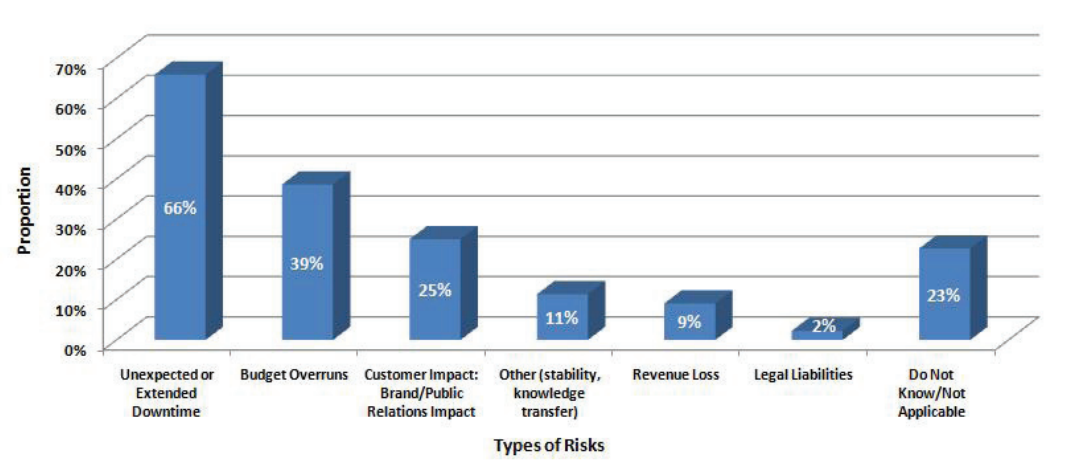
\includegraphics[width=13cm]{images/hitachi_survey}
  \caption{Perceived risk in data migration \cite{paper:hitachi} }
  \label{fig:cpim-nosql}
\end{figure}

\noindent However migrating data between database without causing application downtime brings several new problems such as data synchronization between the two involved systems.

\subsection{Hegira integration}
To mitigate those problems we want to extend the CPIM library to make it able to interact with \textit{Hegira} a migration system able to perform interoperable data migration and synchronization across column-based NoSQL databases \cite{paper:modaclouds-deliverable}. \textit{Hegira} is already able to migrate data offline, but in many cases this solution is not acceptable since this requires to turn off the application for a period of time that depends on the volume of data that needs to be migrated towards the new database. 
Downtime costs and risks of data loss can be problematic so, \textit{Hegira} was extended to be able to perform a live-migration of the data by keeping them synchronized on the source and the destination database.
This feature needs to be exploited at application level and thus we decided to embed it inside the CPIM NoSQL service, in order to make it as transparent as possible to the user.

\noindent The CPIM library needs to be aware of the state of both the synchronization and migration systems and acts accordingly intercepting user operation and sending data manipulation queries (DMQ) to the migration system which is in charge of keeping the data consistent across the replicated databases.

\noindent The result of such integration in the CPIM library will be the ability of the user to migrate data from a NoSQL storage to another, while the application is running, and still be able to read the data on the new system without modifying the application code